% !TEX encoding = UTF-8

%% Davide Imola - VR386238
%% Andre Slemer - VR386253
%% Esame di Linguaggi

\documentclass[a4paper,titlepage]{book}

\usepackage[italian]{babel}
\usepackage[noadvisor]{frontespizio}
\usepackage{amsmath,amssymb,graphicx}
\usepackage{natbib}
\usepackage{url}
\usepackage{float}
\usepackage[T1]{fontenc}

\begin{document}

\pagestyle{plain}

%Generazione Frontespizio
\begin{frontespizio}
\Universita{Verona}
\Dipartimento{Informatica}
\Corso[Laurea]{Informatica}
\Annoaccademico{2016--2017}
\Titoletto{}
\Titolo{Relazione di Linguaggi}
\Sottotitolo{}
\Candidato[VR386238]{Davide Imola}
\Candidato[VR386253]{Andrea Slemer}
\end{frontespizio}

\frontmatter
\tableofcontents

\mainmatter
\chapter{Testo elaborato}
Estendere l'interprete OCAML studiato durante le lezioni del corso di Linguaggi scegliendo una delle tre semantiche studiate:
operazionale, denotazionale o iterativa.
La soluzione dovr\'a contenere il codice base imperativo e funzionale di blocchi, procedure e funzioni.

L'estensione del linguaggio didattico dovr\'a prevedere:
\begin{itemize}
\item Il tipo stringa di caratteri: string
\item La costante string nella semantica come sequenza di caratteri alfanumerici
\item Il calcolo della lunghezza di una stringa: len x
\item La concatenazione di stringhe: s1@s2
\item L'operazione di sottostringa: subs (string, index1, index2)
\end{itemize}

La possibilit\'a di introdurre ulteriori estenzioni/operazioni prendendo ispirazione da operazioni note in linguaggi di scripting
\'e lasciata allo studente.

L'estensione prevede anche l'implementazione del comando 'Reflect string', il quale riceve in input come unico parametro
una stringa e richiama l'interprete sulla stringa, la quale viene vista come sequenza di comandi eseguibili.

\clearpage
\thispagestyle{empty}

\chapter{Struttura del programma}
L'interprete utilizza una semantica denotazionale.
Per rendere pi\'u efficente l'invocazione dell'interprete in fase di testing, abbiamo utilizzato un file di supporto chiamato 'main.ml',
il quale ha il compito di richiamare tutte le parti dell'interprete che risiedono in file diversi:

\section{Linguaggio funzionale}
Abbiamo adottato per una prima stesura del programma un linguaggio funzionale.
La scelta ci ha permesso di costruire una prima versione dell'elaborato finale in modo agevole, in quanto il linguaggio
funzionale permette una più semplice e facile individuazione degli errori.
Per un limite della struttura non siamo riusciti a portare a termine l'elaborato, poich\'e la funzione 'Reflect string' richiedeva che la
stringa ricevuta in ingresso fosse interpretata come sequenza di comandi, il che \'e incompatibile con la struttura del
linguaggio funzionale.

\section{Linguaggio imperativo}
Abbiamo continuato lo sviluppo del software usando un linguaggio imperativo e, riuscendo a trasporre il software funzionale 
prodotto, abbiamo avuto una base di partenza per l'elaborato finale.

\begin{figure}[H]
\center
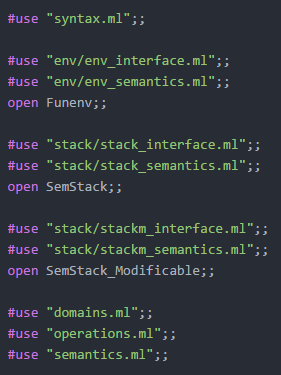
\includegraphics[height=250px]{img/main_funzionale.png}
\caption{Caso funzionale: 'main.ml' \label{fig:main_funzionale}}
\end{figure}

\begin{figure}[H]
\center
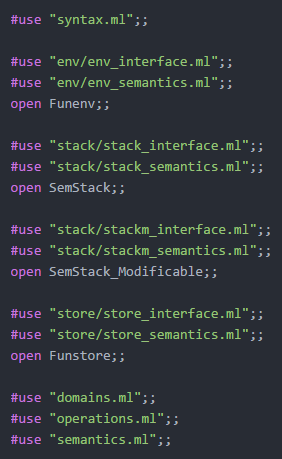
\includegraphics[height=270px]{img/main_imperativo.png}
\caption{Caso imperativo: 'main.ml' \label{fig:main_imperativo}}
\end{figure}

\section{Struttura files del software}
\begin{itemize}
\item \textbf{syntax.ml:} contiene i domini sintattici e definisce la sintassi di tutte le operazioni e i comandi definiti.
\item \textbf{env\_interface.ml:} contiene la signature dell'ambiente.
\item \textbf{env\_semantics.ml:} contiene l'implementazione dell'interfaccia dell'ambiente, definita in \textit{env\_interface.ml}.
\item \textbf{stack\_interface.ml:} contiene la signature dello stack \textbf{non modificabile}.
\item \textbf{stack\_semantics.ml:} contiene l'implementazione dell'interfaccia dello stack \textbf{non modificabile}, definita in \textit{stack\_interface.ml}.
\item \textbf{stackm\_interface.ml:} contiene la signature dello stack \textbf{modificabile}.
\item \textbf{stackm\_semantics.ml:} contiene l'implementazione dell'interfaccia dello stack \textbf{modificabile}, definita in \textit{stackm\_interface.ml}.
\item \textbf{store\_interface.ml:} contiene la signature della memoria.
\item \textbf{store\_semantics.ml:} contiene l'implementazione dell'interfaccia della memoria, definita in \textit{store\_interface.ml}.
\item \textbf{domains.ml:} contiene i domini semantici (esprimibili \textit{eval}, dichiarabili \textit{dval}, memorizzabili \textit{mval}) e le conversioni di tipo.
\item \textbf{operations.ml:} contiene l'operazione \textit{typecheck}, usato per verificare il tipo dei parametri in ingresso ad ogni operazione, e l'implementazione tutte le altre operazioni divise per tipologia (Operazioni \textit{base}, Operazioni sulle \textit{stringhe}, Operazioni di supporto private e non disponibili all'esecuzione, Operazione \textit{parser} e \textit{parserCom} di supporto al comando \textit{Reflect}).
\item \textbf{semantics.ml:} contiene la definizione della semantica di ogni parte sintattica necessaria all'interprete.
\end{itemize}

\clearpage
\thispagestyle{empty}

\chapter{Modifiche al software di base}

\section{Tipo stringa: inserimento}
Per soddisfare l'inserimento del tipo \textbf{stringa} \'e stato aggiunto sia nella sintassi (all'interno del tipo \textit{exp}) e anche
nella semantica (all'interno di tutti e tre i tipi presenti nel file \textit{domains.ml}).

\begin{figure}[H]
\center
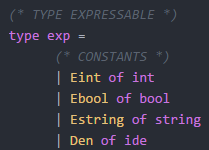
\includegraphics[height=100px]{img/type_exp.png}
\caption{String nel tipo exp: 'syntax.ml' \label{fig:type_exp}}
\end{figure}

\begin{figure}[H]
\center
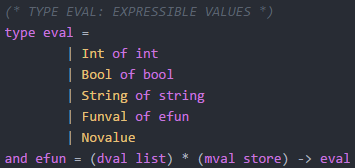
\includegraphics[height=100px]{img/type_eval.png}
\caption{String nel tipo eval: 'domains.ml' \label{fig:type_eval}}
\end{figure}

\clearpage
\section{Tipo stringa: operazioni}

Tutte le operazioni sulle espressioni sono state implementate nel file \textit{operazioni.ml} il quale contiene:
\begin{itemize}
\item Una funzione che implementa il check di tipo, il quale prevede il controllo di tre tipologie di dato: \textit{int}, \textit{bool} e
\textit{string}.

\begin{figure}[H]
\center
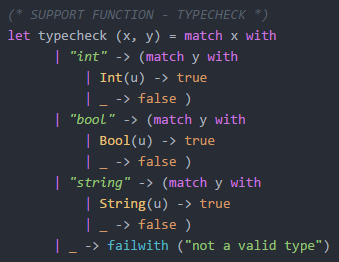
\includegraphics[height=200px]{img/typecheck.png}
\caption{Funzione Typecheck: 'operations.ml' \label{fig:typecheck}}
\end{figure}

\item Una operazione \textbf{'len string'} che restiusce un intero che rappresenta il valore della lunghezza della stringa passata come parametro.
Per lo sviluppo di questa funzione abbiamo fatto affidamento alla funzione \textbf{String.length} di OCaml.

\begin{figure}[H]
\center
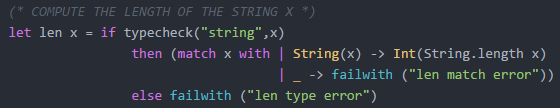
\includegraphics[height=70px]{img/len.png}
\caption{Funzione Len: 'operations.ml' \label{fig:len}}
\end{figure}
\clearpage

\item Una operazione \textbf{'conc string string'} che restituisce una stringa, la quale \'e la concatenazione delle due stringhe passate come parametri.
Per lo sviluppo di questa funzione abbiamo fatto affidamento alla funzione \textit{String.concat} di OCaml, questo ci ha permesso di giustapporre due stringhe inserendole in una lista, utilizzando come stringa di separazione la \textbf{stringa vuota ""}.

\begin{figure}[H]
\center
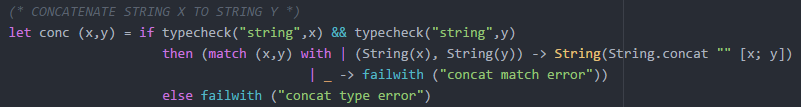
\includegraphics[height=50px]{img/conc.png}
\caption{Funzione Conc: 'operations.ml' \label{fig:conc}}
\end{figure}

\item Una operazione \textbf{'subs string int int'} che restituisce una stringa, la quale \'e composta dal pezzo di stringa passata come parametro che intercorre dal carattere in posizione del primo intero (compreso), fino al carattere in posizione del secondo intero (non compreso).
Per lo sviluppo di questa funzione abbiamo fatto affidamento alla funzione \textbf{String.sub} di OCaml, questo ci ha permesso di evitare molti controlli sull'idoneit\'a dei tre parametri ricevuti in ingresso.

\begin{figure}[H]
\center
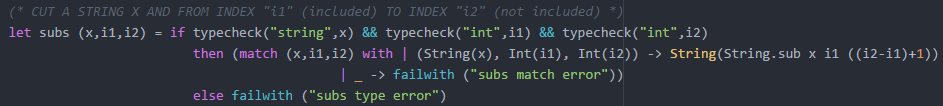
\includegraphics[height=50px]{img/subs.png}
\caption{Funzione Subs: 'operations.ml' \label{fig:subs}}
\end{figure}
\clearpage

\item Una operazione \textbf{'charat string int'} che restitusce un carattere, il quale \'e estratto dalla stringa passata come parametro e risiede nella posizione indicata dall'intero. Il carattere viene memorizzato comunque in formato \textit{String}.

\begin{figure}[H]
\center
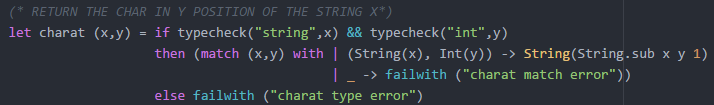
\includegraphics[height=60px]{img/charat.png}
\caption{Funzione CharAt: 'operations.ml' \label{fig:charat}}
\end{figure}

\item Una operazione \textbf{'streq string string'} che restituisce un valore \textit{'boolean'}, il quale \'e calcolato confrontando le due stringhe passate come parametro. Viene utilizzato come supporto la funzione \textit{'String.compare'} la quale restiusce un valore intero (\textit{negativo} se x < y, \textit{uguale a zero} se x = y, o \textit{positivo} se x > y).

\begin{figure}[H]
\center
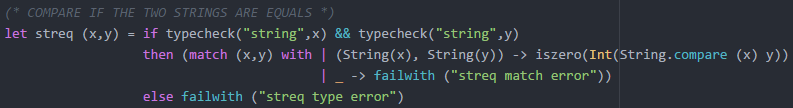
\includegraphics[height=55px]{img/streq.png}
\caption{Funzione StrEq: 'operations.ml' \label{fig:streq}}
\end{figure}
\end{itemize}
\clearpage

\section{Comando Reflect}
Il comando \textbf{'Reflect string'} riceve in ingresso una stringa e la interpreta come una sequenza di \textit{espressioni} e \textit{comandi}, richiamando su di essa l'interprete stesso.

Reflect permette di effettuare uno scan della stringa da sinistra a destra, eseguendo ogni token riconosciuto come comando o espressione ed aspettandosi dopo ogni sotto-stringa riconosciuta i parametri definiti nella semantica corrispondente.

Il comando \'e stato implementato nella semantica dei comandi il quale controlla che la stringa sia formattata correttamente controllando che il numero di parentesi \textbf{'('} e \textbf{')'} sia di egual numero, inoltre controlla se il primo token della stringa rappresenta un comando o un'espressione.

Nel caso la funzione \textit{'isCommand()'} dovesse riconoscere un comando \textit{(restituendo un boolan con valore 'true')}, verrebbe invocata la funzione \textit{parserCom()}, altrimenti verrebbe richiamata la funzione \textit{parser}.

Per visualizzare il risultato viene allocata e dichiarata una variabile di output, chiamata \textit{"result"}.

\begin{figure}[H]
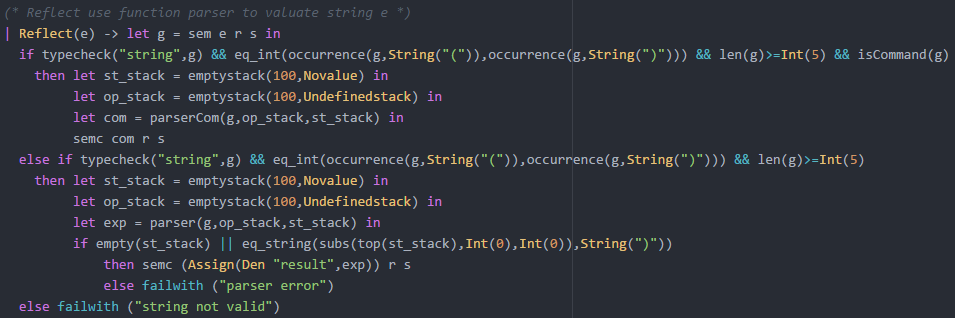
\includegraphics[height=150px]{img/reflect.png}
\caption{Comando Reflect: 'semantics.ml' \label{fig:reflect}}
\end{figure}

\section{Parser}
La funzione \textit{parser} ha bisogno di tre parametri:

\begin{figure}[H]
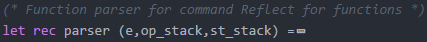
\includegraphics[height=40px]{img/parser.png}
\end{figure}

\begin{itemize}
\item \textbf{e:} contiene la stringa che il parser deve analizzare.
\item \textbf{op\_stack:} contiene i token che vengono riconosciuti come espressioni e non sono ancora stati eseguiti.
\item \textbf{st\_stack:} contiene il resto della stringa che deve essere ancora analizzato.
\end{itemize}
\clearpage
La soluzione implementata scansiona la stringa in modo sequenziale.

La funzione riconosce i vari token grazie ad una funzione di \textit{'substring'} che punta sempre a leggere la prima parola della stringa rimanente.

\textbf{Caso base:} la funzione incontra la fine della stringa o un tipo terminale \textit{(Den, Eint, Ebool, Estring)}

\textbf{Caso ricorsivo:} la funzione incontra un'espressione che necessita di uno o pi\'u parametri. In questo caso il token viene memorizzato e si procede a successive scansioni per la lettura dei parametri. Solo quando tutti i parametri sono stati letti correttamente l'espressione viene eseguita.

\section{ParserCom}
La funzione \textit{parserCom} utilizza gli stessi tre paramteri della funzione \textit{parser}, ma viene chiamata ogni volta che viene riconosciuto che il primo token della stringa \textbf{e} \'e un comando.

\chapter{Esempi}

\end{document}